\chapter[2021 May]{May 2021}

\section[2021/05/03]{Monday, 3 May 2021}

\subsection{Experimental Plan}

This section presents the inital draft of the experimental plan required to demonstrate conformance to the system specifications. Prior to the commencement of any of the qualification tests, the following setup steps must have been completed:

\begin{compactenum}
    \item Ensure robotic manipulator's workspace is completely empty.
    \item Power on the PC that will run the system control software.
    \item Ensure the system camera has a clear view of the system workspace and connect the camera to the PC.
    \item Connect the robotic subsystem to the PC.
    \item Power on the robotic subsystem.
    \item Start the system control software on the PC and verify a connection is established with the camera and robotic subsystem.
    \item Initialise the system calibration process using the system control software GUI and verify the calibration completes successfully.
\end{compactenum}

The following 3D shapes are defined for use in multiple qualification tests (where the dimensions are in number of cubes):

\begin{compactenum}
        \item A cube consisting of three 3 x 3 layers.
        \item A pyramid with a 4 x 4 square base which is followed by a 3 x 3 layer, 2 x 2 layer and finally a single cube in the top layer.
        \item A pyramid with a 4 x 4 square base similar to the above pyramid, but with the 3 x 3 layer rotated 20 degrees clockwise relative to the layer below and both the 2 x 2 layer and top layer rotated 45 degrees relative the layer below.
\end{compactenum}

\subsubsection*{Qualification Test 1: Test of system's capability to facilitate the definition of 3D shapes}

\paragraph{\textit{Test Objectives}} 

The aim of this test is to determine if the system is capable of capturing and representing a user-specified 3D shape where the position of each constituent cube is specified along each Cartesian axis as well as the orientation about the z-axis.

\paragraph{\textit{Equipment}} 

Only the final 3D shape cube construction system is required for this test.

\paragraph{\textit{Experimental Parameters and Setup}}

Prepare for the qualification test by navigating to the 3D shape definition screen in the system control GUI.

\paragraph{\textit{Experimental Protocol}}

Complete the following steps to execute the qualification test:

\begin{compactenum}
    \item Select one of the test shapes defined above to input into the system.
    \item Input the Cartesian position and orientation of each cube into system control software.
    \item Once all of the cubes have been defined in the software, compare the captured Cartesian position and orientation with the desired values.
    \item Verify the 3D render of the test shape shown in the GUI correctly represents the test shape.
    \item Repeat all the steps 1 to 4 of the experimental protocol with a different test shape selected in step 1.
    \item Repeat step 5 until all the test shape definitions have been captured by the system.
\end{compactenum}

\subsubsection*{Qualification Test 2: Test of the system's capability to build 3D shapes}

\paragraph{\textit{Test Objectives}}

The aim of this test is to determine if the system is capable of constructing a variety of novel and moderately complex 3D shapes using small cubes each with a side length of between 10mm and 15mm. Novel and moderately complex 3D shapes consitute shapes containing up to at least 30 cubes where each cube has a face parallel to the base plane.

\paragraph{\textit{Equipment}} 

The following items are required for this qualification test:

\begin{compactitem}
    \item Final 3D shape cube construction system
    \item 30 cubes all with side lengths equal and between 10mm and 15mm
\end{compactitem}

\paragraph{\textit{Experimental Parameters and Setup}}

Complete the following steps to prepare for the qualification test:

\begin{compactenum}
    \item Navigate to the 3D shape selection screen for pre-defined shapes in the system control GUI.
    \item Verify the test shapes are available for selection as pre-defined shapes in the system control software.
\end{compactenum}

\paragraph{\textit{Experimental Protocol}}

Complete the following steps to execute the qualification test:

\begin{compactenum}
    \item Clear the robitc manipulator's workspace and insert the 30 cubes into the system loading mechanism.
    \item Select a pre-defined test shape in the system control GUI.
    \item Start the construction process in the system control GUI and wait for the robotic subsystem to construct the shape.
    \item Compare the constructed shape to the selected pre-defined test shape in the GUI.
    \item Repeat all the steps 1 to 4 of the experimental protocol with a different pre-defined test shape selected in step 2. 
    \item Repeat step 5 until all the pre-defined test shapes have been built.
\end{compactenum}

\subsubsection*{Qualification Test 3: Test of end-effector's capability to manipulate cubes}

\paragraph{\textit{Test Objectives}}

The aim of this test is to determine if the end-effector is capable of maintaining a cube in its grip under motion when the robotic manipulator is at maximum acceleration. The test also aims to determine if the end-effector is able to maintain the cube in its grip for at least 20 seconds continuously and if it is able to grip and ungrip the cube.

\paragraph{\textit{Equipment}}

The following items are required for this qualification test:

\begin{compactitem}
    \item Final 3D shape cube construction system
    \item 1 cube with a side length between 10mm and 15mm
\end{compactitem}

\paragraph{\textit{Experimental Parameters and Setup}} 

Complete the following steps to prepare for the qualification test:

\begin{compactenum}
    \item Navigate to the system test screen in the GUI.
    \item Place the cube flat at an arbitraty location on the base plane in the robotic manipulator's workspace.
\end{compactenum}

\paragraph{\textit{Experimental Protocol}}

Complete the following steps to execute the qualification test:

\begin{compactenum}
    \item Initiate the routine for qualification test 3 in the GUI.
    \item Verify the robotic subsystem proceeds to locate and grip the cube placed during the test setup.
    \item Verify the robotic subsystem continously moves the cube between the extremes on all axes for a period of 20 seconds as indicated by the timer in the GUI.
    \item Verify the robotic subsystem places the cube back on the base plane and releases the cube.
\end{compactenum}

\subsubsection*{Qualification Test 4: Measurement of robotic manipulator accuracy}

\paragraph{\textit{Test Objectives}}

The aim of this test is to determine the linear repeatability of the robotic manipulator's positioning along each Cartesian axis as well as its rotational repeatability about the z-axis.

\paragraph{\textit{Equipment}}

The following items are required for this qualification test:

\begin{compactitem}
    \item Final 3D shape cube construction system
    \item Digital depth gauge caliper
    \item Digital height gauge caliper
    \item Digital protractor
    \item Piece of paper
    \item Thin plastic disc with an 10mm diameter custom designed to attach to the end-effector. This purpose of this disc is to increase the measurement resolution of the end-effector's rotation.
\end{compactitem}

\paragraph{\textit{Experimental Parameters and Setup}}

Prepare for the qualification test by navigating to the system test screen in the GUI.

\paragraph{\textit{Experimental Protocol}}

Complete the following steps to execute the qualification test:

\begin{compactenum}
    \item Initiate the routine for qualification test 4 for the x an y axes in the GUI.
    \item The robotic manipulator will move the end-effector to an arbitrary location on the base plane. Measure the perpendicular distance from the nearest edge of the workspace to the nearest point on the end-effector in both the x and y directions using the digital depth gauge caliper.
    \item Instruct the system to continue with the test in the GUI. The robotic manipulator will return to the origin of the x and y axes before returning to approximately the same point as in the step above.
    \item Take another measurement as in step 2.
    \item Repeat steps 3 and 4 until 5 measurements have been taken for both the x and y axes.
    \item Initiate the routine for qualification test 4 for the z axis in the GUI.
    \item The robotic manipulator will move the end-effector to an arbitrary location in 3D space. Measure the perpendicular distance from the base plane of the workspace to the nearest point on the end-effector in the z direction using the digital height gauge caliper.
    \item Instruct the system to continue with the test in the GUI. The robotic manipulator will return to the origin of the z axis before returning to approximately the same point as in the step above.
    \item Take another measurement as in step 7.
    \item Repeat steps 7 and 8 until 5 measurements have been taken.
    \item Attach the plastic disc to the end-effector and place the paper on the base plane.
    \item Initiate the routine for qualification test 4 for rotation about the z axis in the GUI.
    \item The robotic manipulator will move the end effector to an arbitrary location on the paper with the end-effector aligned with the rotational origin. Mark the rotational position of the disc on the paper.
    \item Instruct the system to continue with the test in the GUI. The robotic manipulator will rotate the end-effector an arbitrary amount.
    \item Mark the rotational position of the disc on the paper and measure the rotational angle using the digital protractor.
    \item Instruct the system to continue with the test in the GUI. The robotic manipulator will rotate back to the rotational origin and return to approximately the same rotational orientation.
    \item Repeat steps 15 and 16 until 5 measurements have been taken.
\end{compactenum}

\subsubsection*{Qualification Test 5: Measurement of computer vison cube detection accuracy}

\paragraph{\textit{Test Objectives}}

The aim of this test is to determine the accuracy of the computer vision system in detecting and localising cubes whose faces are visible from a vertical perspective. Specifically, the test aims to determine the accuracy of the linear localisation along the x-axis and y-axis as well as the rotational pose estimation about the z-axis.

\paragraph{\textit{Equipment}}

The following items are required for this qualification test:

\begin{compactitem}
    \item Final 3D shape cube construction system
    \item 1 cube with a side length between 10mm and 15mm
    \item Digital depth gauge caliper
    \item Digital protractor
\end{compactitem}

\paragraph{\textit{Experimental Parameters and Setup}}

Prepare for the qualification test by navigating to the system test screen in the GUI.

\paragraph{\textit{Experimental Protocol}}

Complete the following steps to execute the qualification test:

\begin{compactenum}
    \item Use the digital protractor and depth gauge caliper to place the cube at a arbitrary known location and orientation on the base plane with respect to the localisation markings on the base plane.
    \item Initiate the routine for qualification test 5 in the GUI. The computer vision subsystem will proceed to detect and localise the cube and display the detected Cartesian position and z-axis rotational orientation.
    \item Compare the detected Cartesian position and z-axis rotational orientation to the actual measured values.
\end{compactenum}

\subsubsection*{Qualification Test 6: Test of system's capability to detect a dropped cube}

\paragraph{\textit{Test Objectives}}

The aim of this test is to determine if the system is capable of detecting when a cube has been dropped by the end-effector.

\paragraph{\textit{Equipment}}

The following items are required for this qualification test:

\begin{compactitem}
    \item Final 3D shape cube construction system
    \item 1 cube with a side length between 10mm and 15mm
\end{compactitem}

\paragraph{\textit{Experimental Parameters and Setup}}

Prepare for the qualification test by placing the cube at an arbitrary location on base plane in the robotic manipulator's workspace.

\paragraph{\textit{Experimental Protocol}}

Complete the following steps to execute the qualification test:

\begin{compactenum}
    \item Initiate the routine for qualification test 6 in the GUI. The robotic subsystem will locate and grip the cube before proceeding to move arbitrarily throughout the 3D workspace.
    \item Instruct the end-effector to release the cube using the GUI. This action will not inform the system that a cube has been dropped.
    \item Wait for the system to detect that a cube has been dropped.
    \item Verify that the system shows a notification on the GUI indicating a dropped cube has been detected.
\end{compactenum}

\pendsign

\section[2021/05/17]{Monday, 17 May 2021}

\subsection{End-Effector Prototype 1}

A vacuum gripper approach was selected for protoyping as the system's end-effector based on earlier research. In order to construct the prototype, the following components were acquired:

\begin{compactitem}
    \item SMC 8mm diameter vacuum pad M5 female thread with adaptor (ZPT08UN-B5).
    \item SMC straight M5 male threaded adaptor to push in 5 mm barb (M-5AU-6).
    \item Through hole guage negative pressure sensor (ADP5111).
    \item 3m x black silicon tubing.
    \item 20ml plastic syringe.
    \item 30 x 12.6mm aluminum cubes.
    \item 4 x plastic t-couplings for tubing.
\end{compactitem}

In order to construct the prototype, the vacuum pad adaptor was attached to the straight barb adaptor using the M5 thread connection. Three pieces of length 20mm, 20mm and 150mm were cut from the silicon tubing and the 150mm length was connected to the straight barb adaptor. The t-coupling was used to connect the other end of the 150mm tube to the other two 20mm tube pieces. The other end of one of the 20mm tube pieces was connected to the syringe and the other to the pressure sensor. Initially, the pressure sesnor nozzle diameter proved to be too narrow to form an airtight seal with the silicon tubing. This was rectified using 3 pieces of heat shrink tubing around the nozzle to increase its diameter. 

The idea behind this construction is to place the vacuum pad on the cube and create a negative pressure within the tubing by pulling out the syringe handle. This negative pressure exerts a force perpendicular to the face of the cube and if the force is great enough the cube remains against the vacuum pad during motion. The cubes were manufactured from a square aluminium extrusion and cut slightly oversize. A CNC machine was used to refine the side lengths of the cubes. Lastly, the cubes were blasted with fine sand to reduce the surface reflectivity as reflective surfaces introduce complications with object recognition. To test that the vacuum system design would be capable of gripping the cubes effectively, even with the slightly uneven sand-blasted cube surface, a test was conducted to test the system's ability to maintain pressure.

\subsection{Pressure Leakage Test}

\subsubsection{Aim}

The aim of this experiment is to quantify the ability of the vacuum system prototype to maintain pressure and the maintain its grip on a aluminium cube.

\subsubsection{Equipment}

The following equipment is required to conduct the experiment:

\begin{compactitem}
    \item End-effector prototype 1.
    \item Arduino Nano microcontroller board.
    \item 1 x 100 nF capacitor.
    \item 1 x 1 nF capacitor.
    \item Breadboard.
    \item Connection wires.
    \item Stand to support the end-effector.
    \item USB Type B Mini to USB Type A connecting wire.
    \item Personal computer.
    \item 1 x 12.6mm aluminium cube.
\end{compactitem}

\subsubsection{Experimental Setup}

The pressure sensor was connected to the 10-bit ADC input of the Arduino Nano using the connecting wires and the breadboard. The capacitors were connected in parallel across the power supply terminals of the pressure sensor. The setup of the circuit on the breadboard is shown in \FigRef{fig:end-effector-circuit-setup}. A C++ program was developed to sample the ADC pressure readings at a sample rate of 1 Hz and transmit them to the PC using a serial connection and a baud rate of 19200. A Python script was developed to log the values received from the Arduino Nano and cease recording when the pressure reached atmospheric levels. \FigRef{fig:end-effector-experimental-setup} shows the experimental-setup of the system. The wooden stand was used as a support to maintain the vacuum pad in mid-air.

\begin{figure}[!ht]
    \centering
    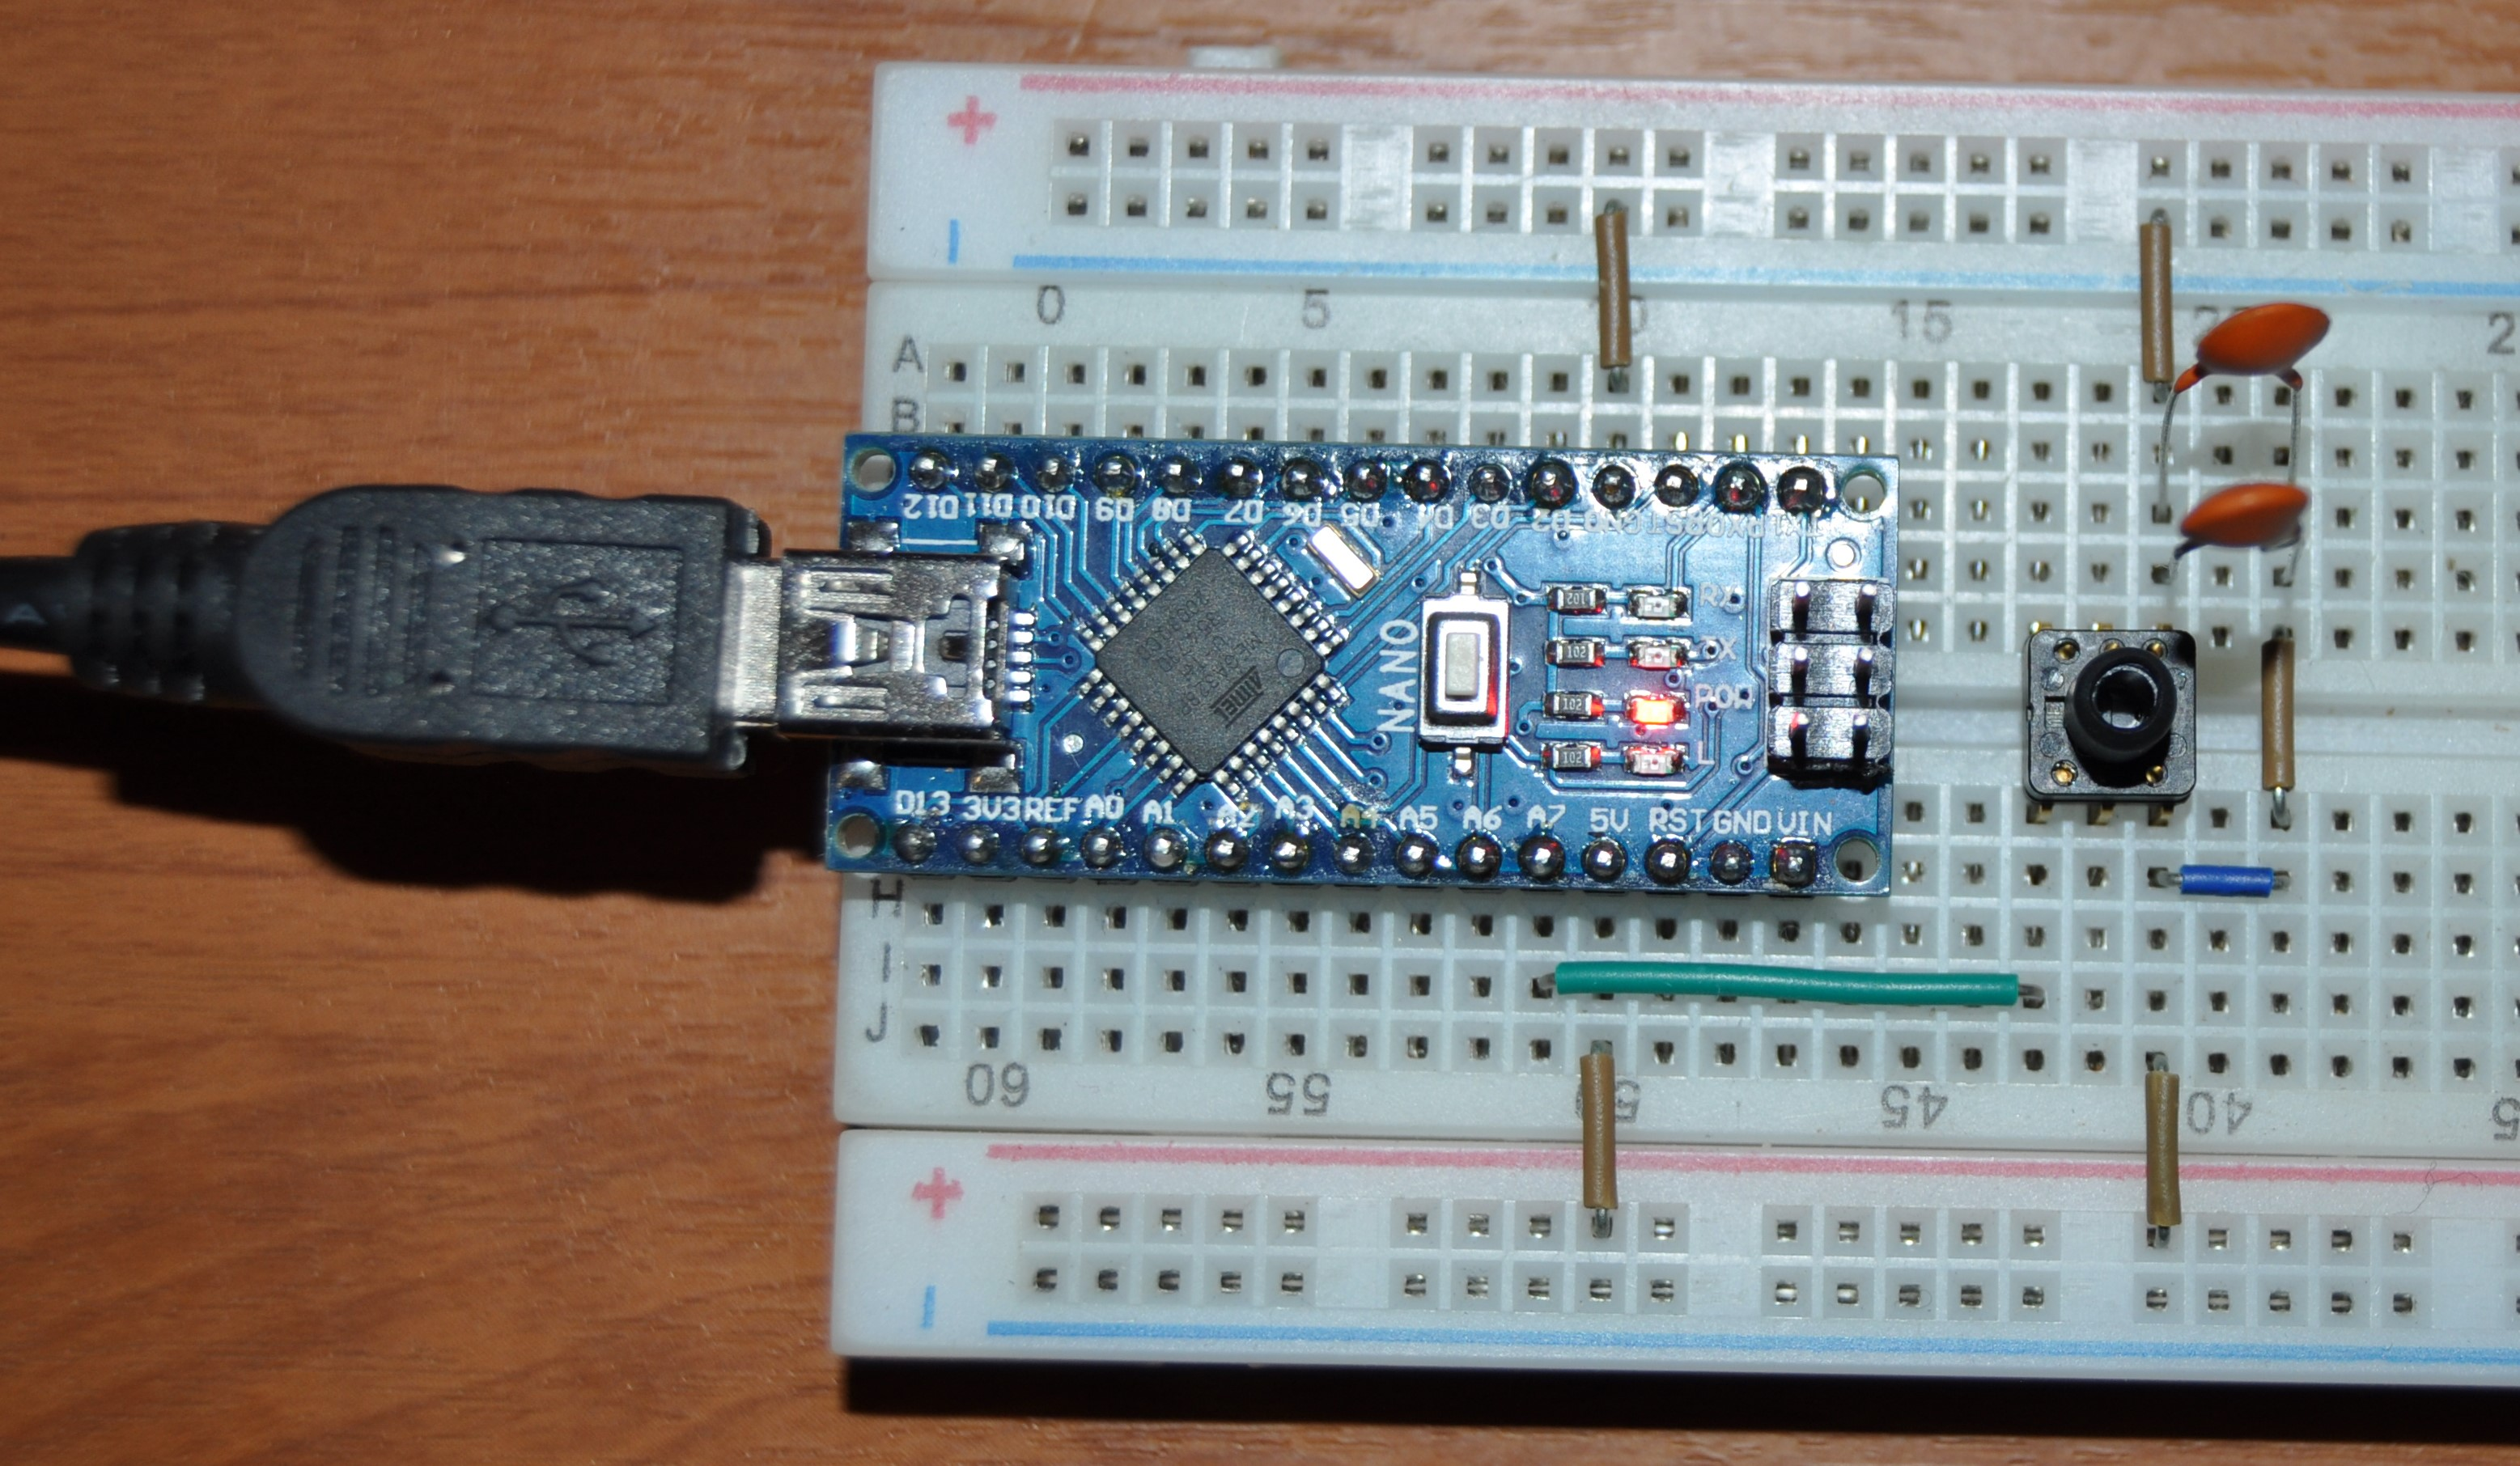
\includegraphics[width=0.6\linewidth]{figures/202105/end-effector-circuit-setup.jpg}
    \caption{Setup of the Arduino Nano and pressure sensor circuit on the breadboard.}
    \label{fig:end-effector-circuit-setup}
\end{figure}

\begin{figure}[!ht]
    \centering
    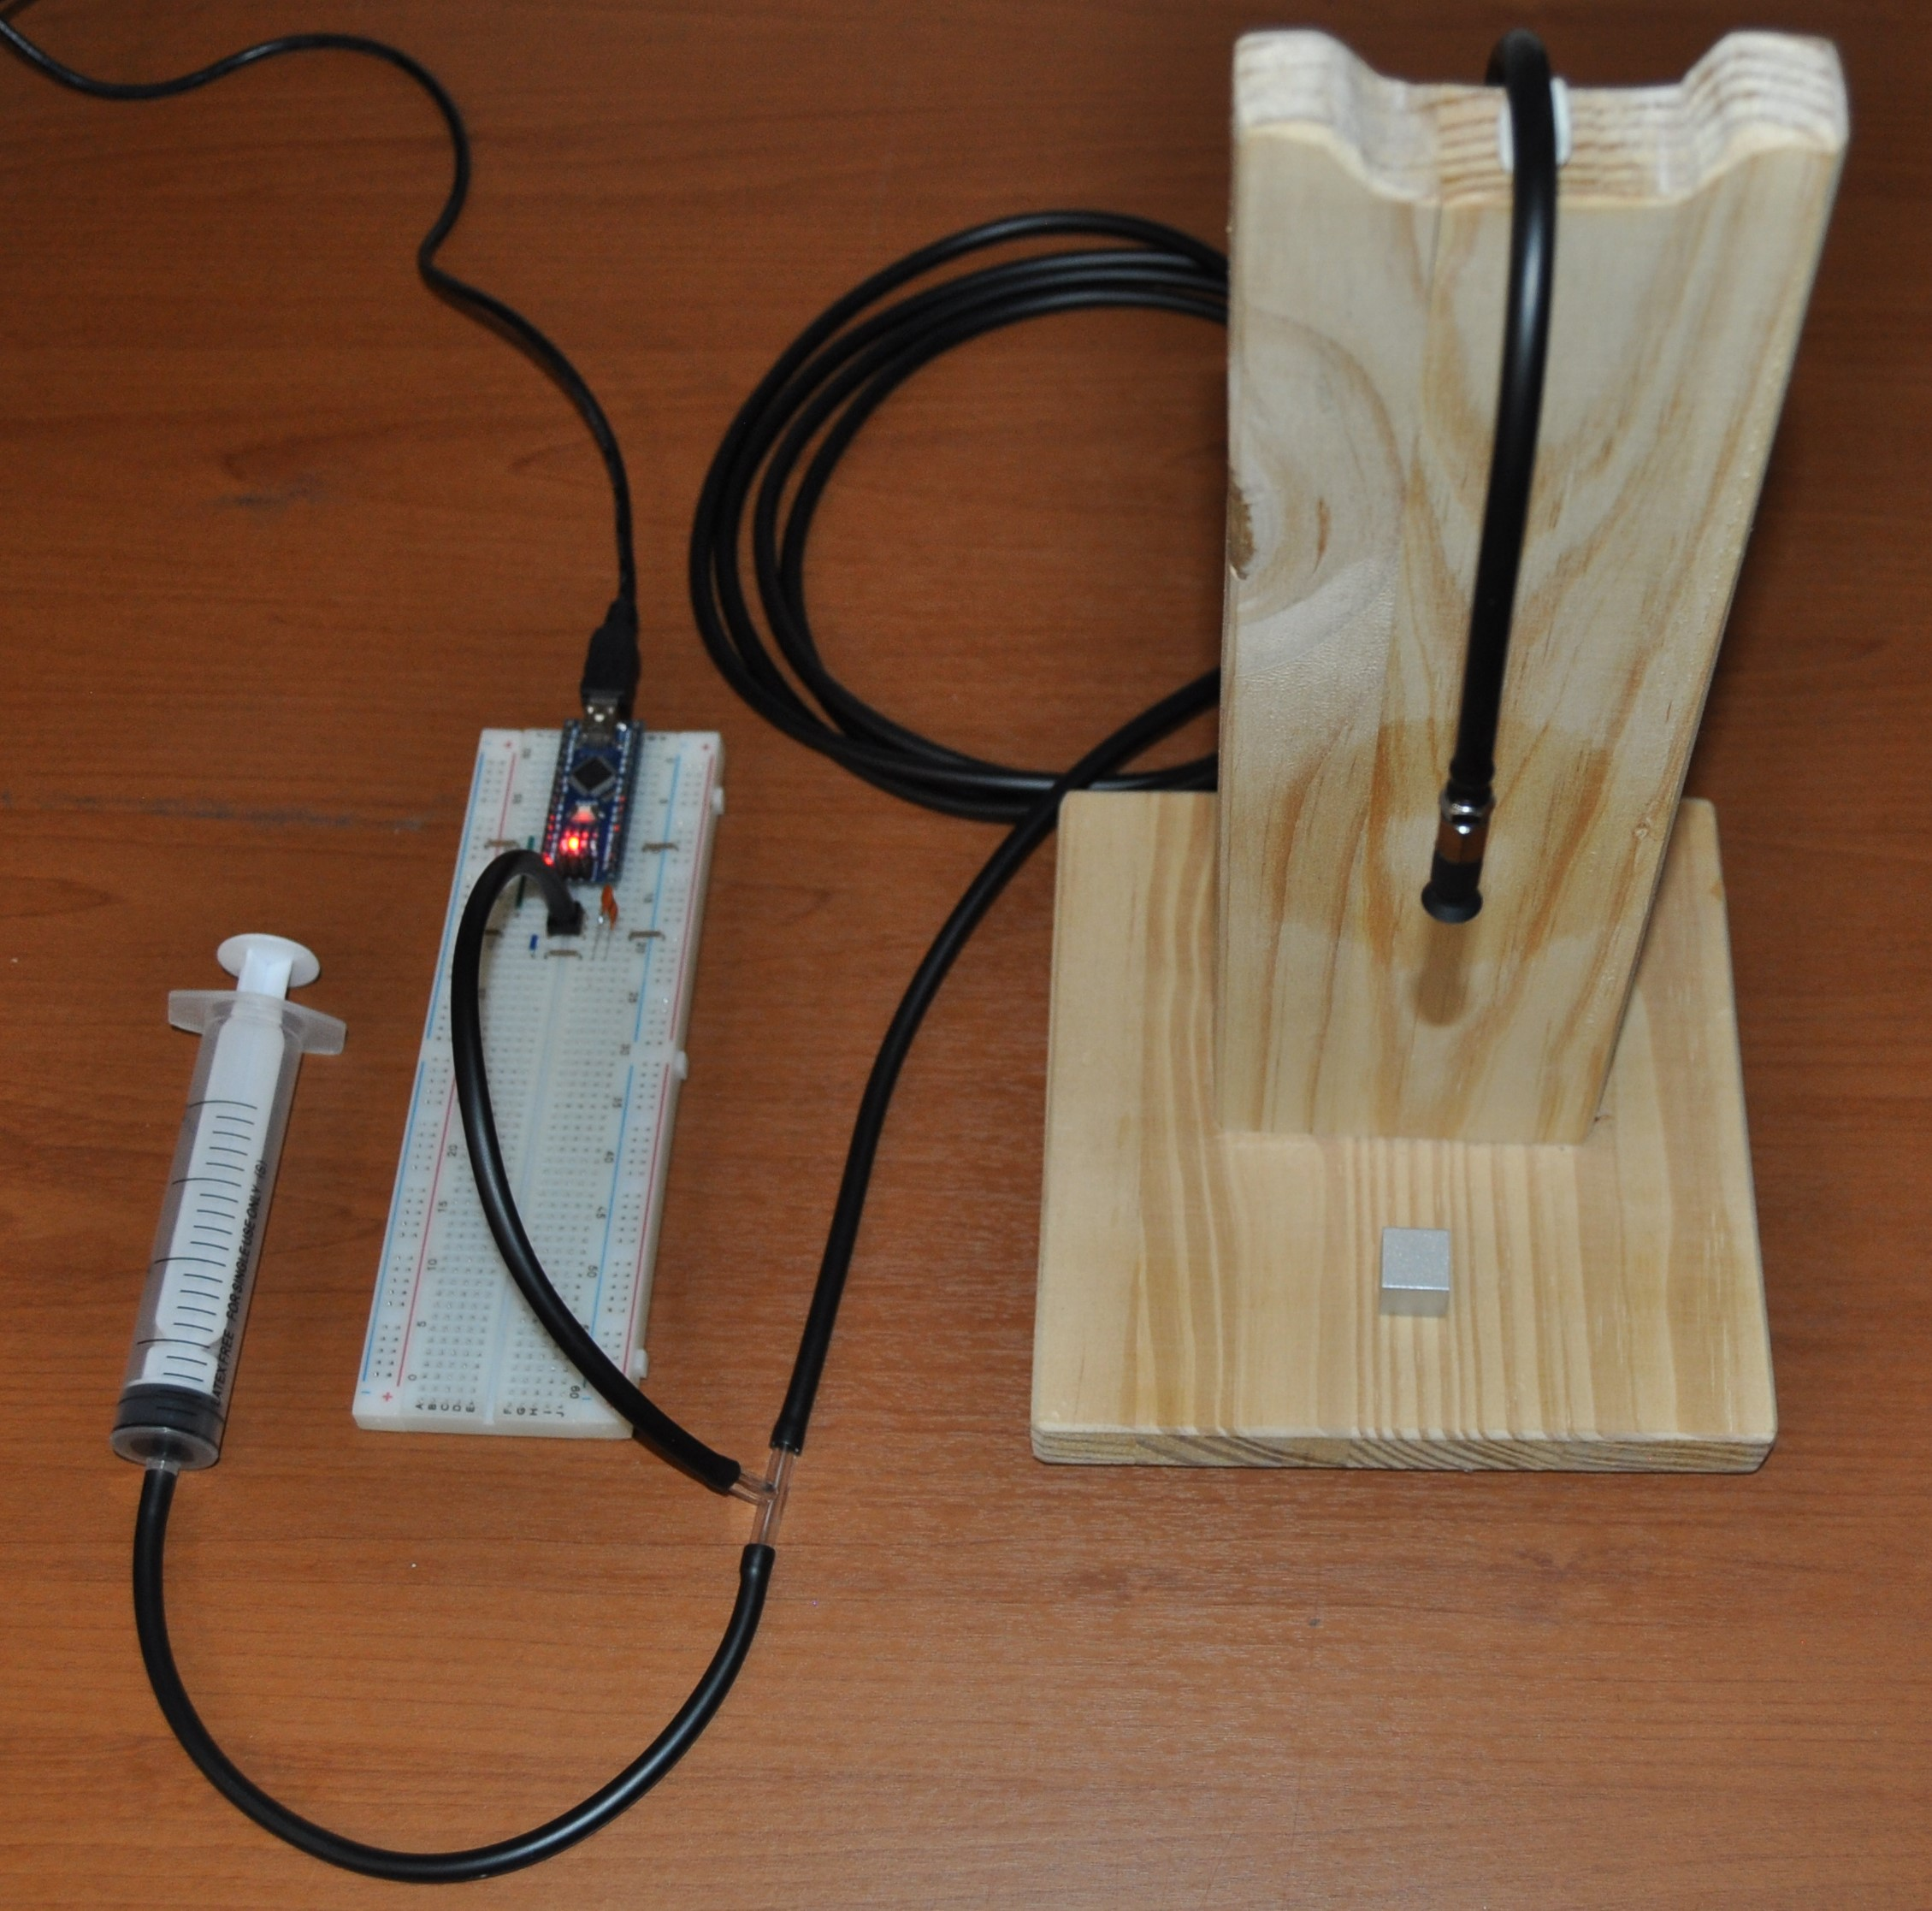
\includegraphics[width=0.6\linewidth]{figures/202105/end-effector-experimental-setup.jpg}
    \caption{The end-effector prototype connected with components required to conduct the pressure leakage experiment.}
    \label{fig:end-effector-experimental-setup}
\end{figure}

\subsubsection{Method}

The following steps were followed to carry out the experiment:

\begin{compactenum}
    \item Hold the cube flush against the bottom of the vacuum pad.
    \item Pull the syringe handle out to maximum extension and verify the vacuum pad grips the cube as shown in \FigRef{fig:end-effector-cube-grip}.
    \item Initiate the Python script to record the pressure readings over time.
    \item When the pressure drops to the extent that the cube drops, verify the Python script terminates.
\end{compactenum}

\begin{figure}[!ht]
  \centering
  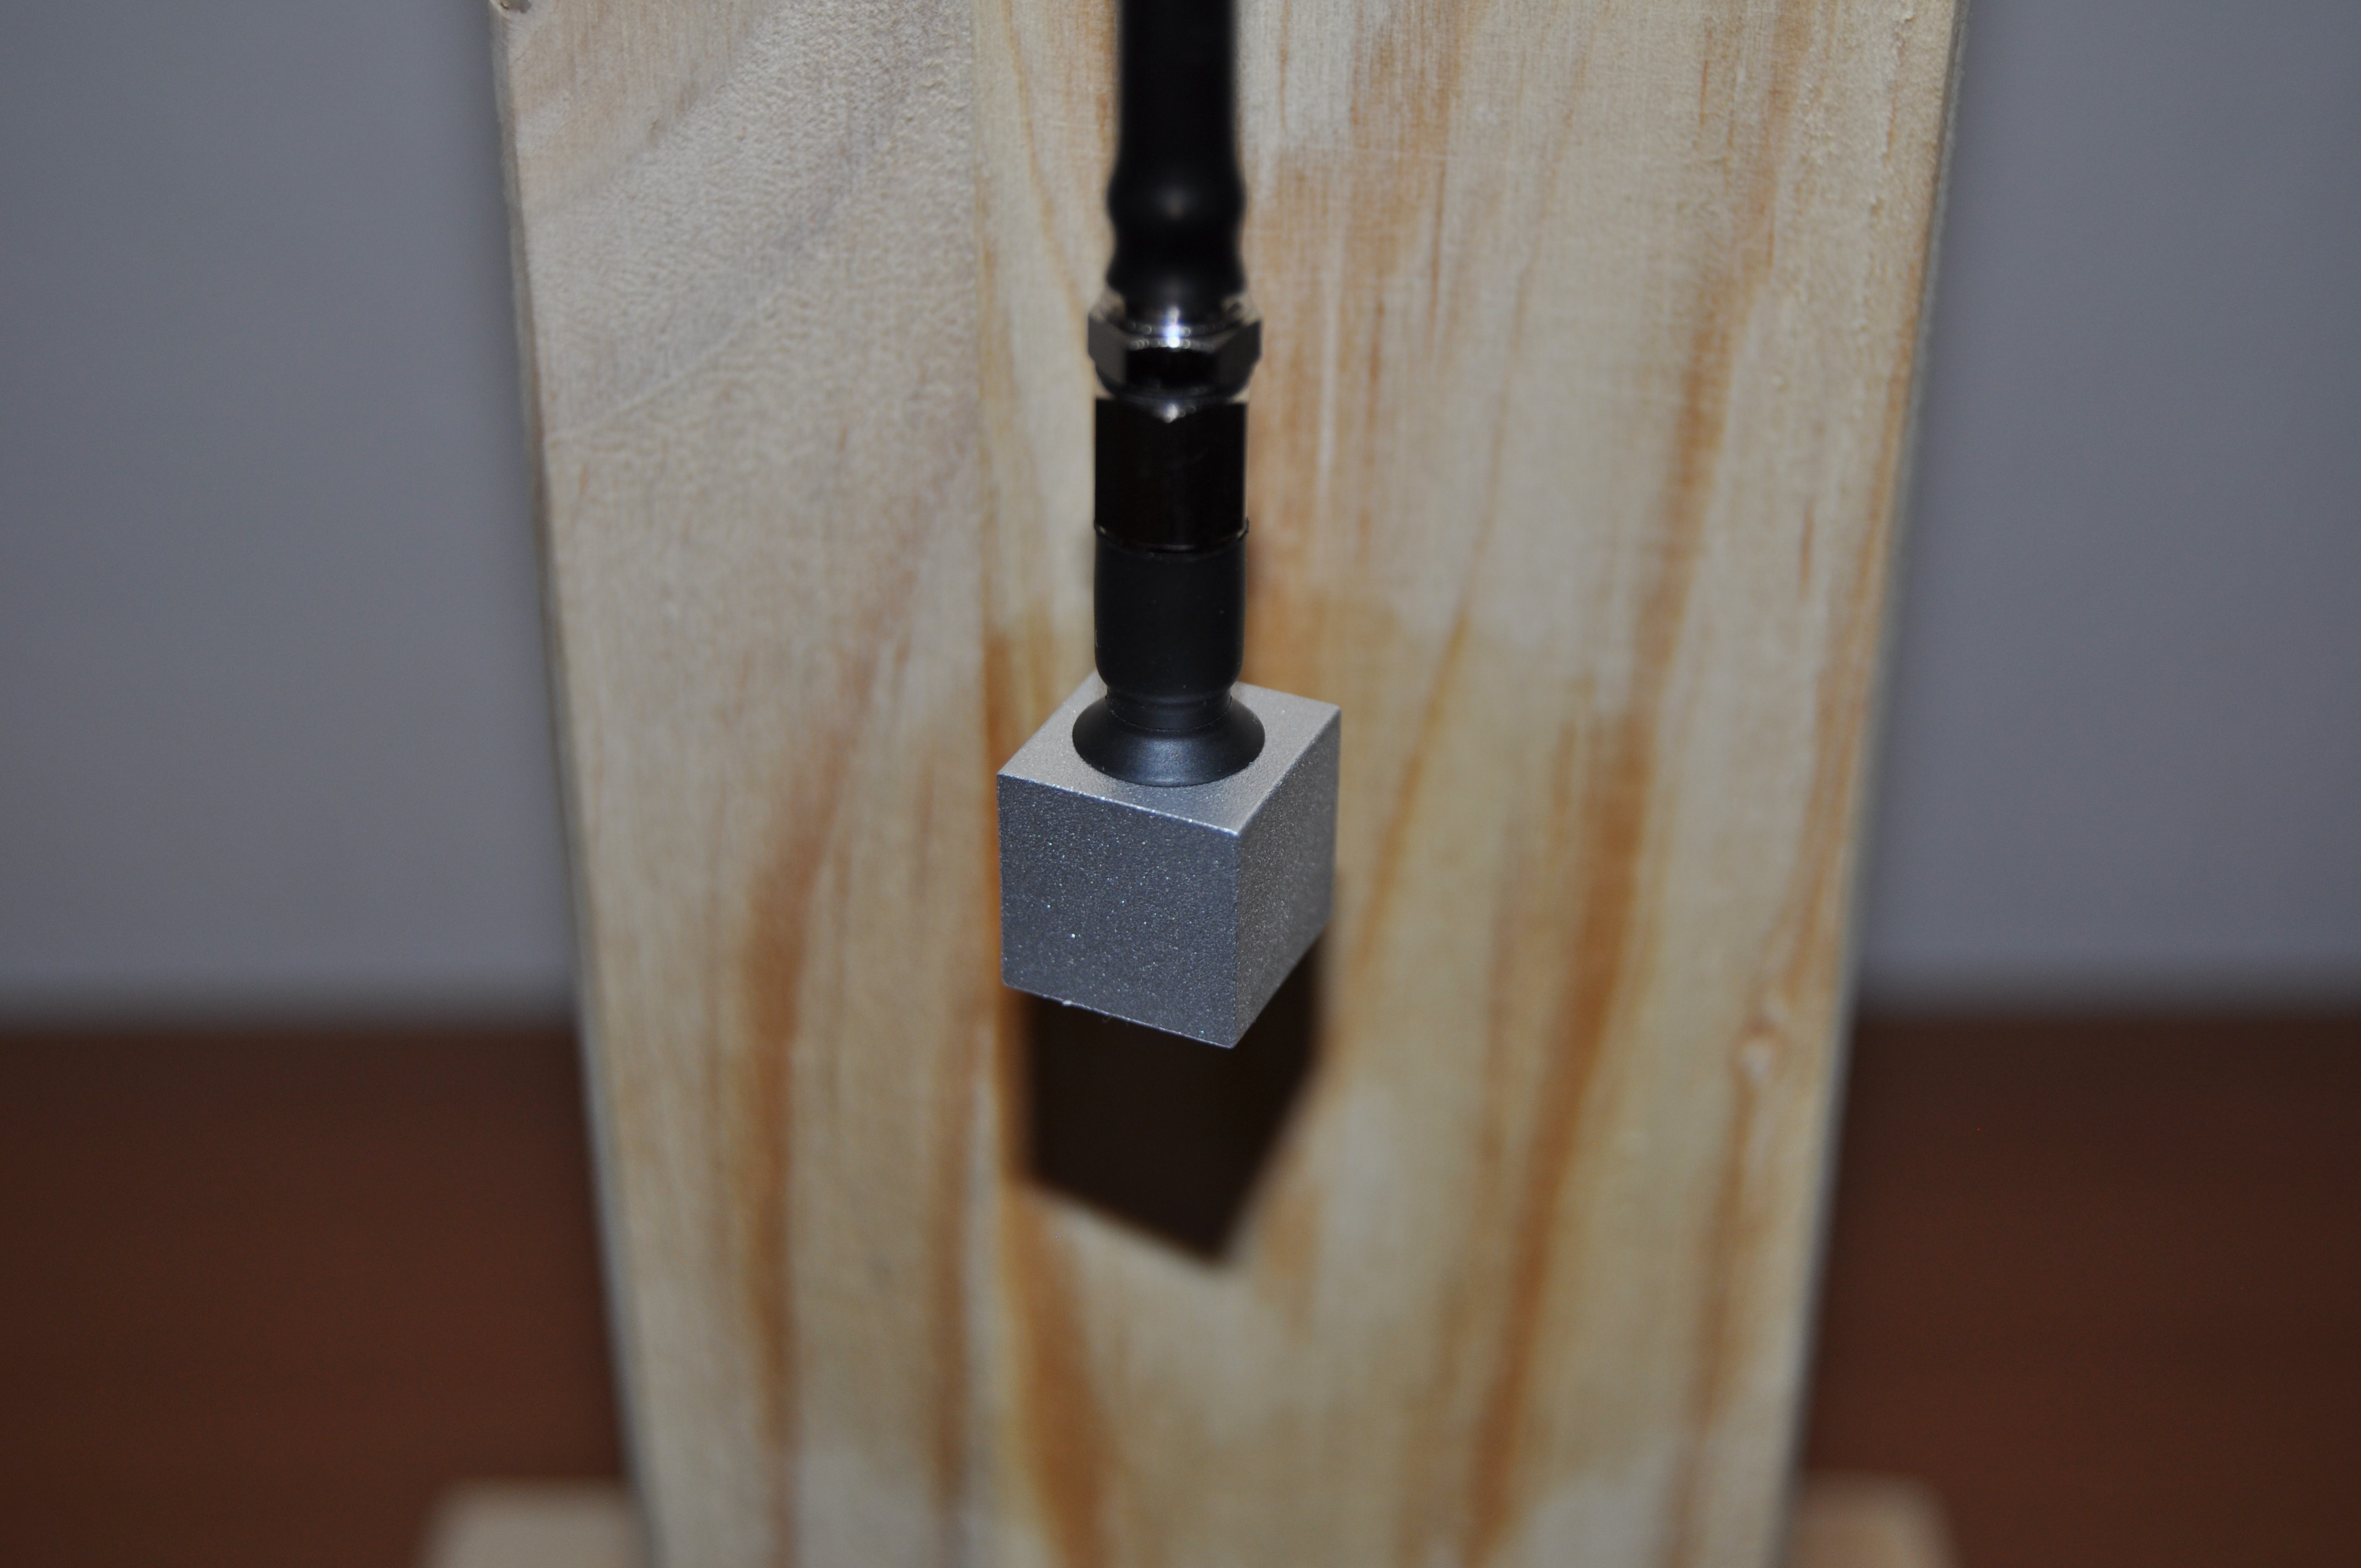
\includegraphics[width=0.6\linewidth]{figures/202105/end-effector-cube-grip.jpg}
  \caption{The vacuum pad and adaptor gripping the aluminium cube when the system contains a pressure significantly lower than atmospheric pressure.}
  \label{fig:end-effector-cube-grip}
\end{figure}

\subsubsection{Results and Discussion}

\FigRef{fig:end-effector-pressure-leak} shows the change in pressure within the vacuum system over time. Since the pressure sensor type is a guage pressure sensor, it measures the relative difference between the atmospheric pressure and the pressure within the system. Since the sesnor is specified as a -100 kPa sensor, the magnitude of the ADC pressure reading is directly proportional to how much lower the internal pressure is compared to the atmospheric pressure. This relative pressure is important as the magnitude of the pressure difference is proportional to the suction force exerted on the cube by the vacuum pad. An ADC reading of 100 corresponds to atmospheric pressure. 

\begin{figure}[!ht]
    \centering
    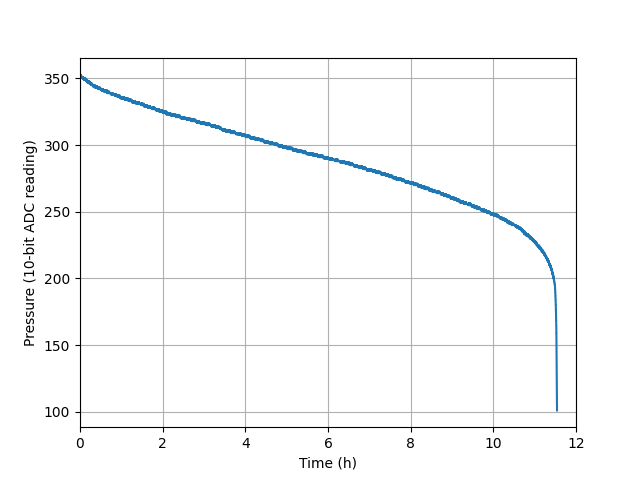
\includegraphics[width=0.7\linewidth]{figures/202105/end-effector-pressure-leak.png}
    \caption{Plot showing the loss of pressure over time within the vacuum system in terms of the raw 10-bit ADC pressure reading. An ADC reading of 100 corresponds to atmospheric pressure and greater readings correspond to lower pressures relative to the atmosphere.}
    \label{fig:end-effector-pressure-leak}
\end{figure}

\FigRef{fig:end-effector-pressure-leak} shows that the system loses pressure at a linear rate over a long period of time. It takes the 10 hours for the reading to drop by 100. However, at 10 hours and a reading of 250, the rate of pressure loss begins to increase exponentially until the loss becomes almost instantaneous at just over 11 hours. This is the point at which the cube was dropped due to insufficient pressure to overcome the weight of the cube. The ability of the system to hold pressure much longer than the required 20 seconds specified in the project proposal indicates it is a good candidate for the end-effector. In order to make a final decision, the system needs to be investigated when greater forces are applied, i.e. when the cube experiences an acceleration.

\pendsign

\section[2021/05/26]{Wednesday, 26 May 2021}

\subsection{Robotic Manipulator Considerations}

The general motor-driven gantry robotic system design is currently the leading option for use in this project's solution. The reasons for this are as follows:

\begin{compactitem}
    \item A gantry-style robotic system offers the most structural stability due to the multiple mounting points for both the frame as well as the moving sub-components within the system. This mechanical stability improves the precision of the system which is one of the leading requirements in this application. It is for this reason that the gantry design is common in other high-precision applications such as pick-and-place operations in circuit manufacturing.
    \item Due to the Cartesian nature of the gantry movement, the precision of the system is relatively constant accross all coordinates in the workspace. This stands in contrast to robotic arms which experience a deterioration in accurary as the distance from the robotic base increases.
    \item The frame of the gantry has the potential to include an integrated mount for the computer vision camera/s. This would allow the camera to always operate from a similar point relative to the workspace and reduce the inaccuracies that are introduced from positional shifts of the camera each time the system is used.
\end{compactitem}

\subsection{Selection of Motor for Prototyping}

In order to drive movement in each of the Cartesian directions, the gantry robotic system requires at least three motors. Furthermore, in order to drive rotation about the z-axis and to drive the end-effector mechanism, an additional two motors are required. The two primary considerations of the motors for this project are the precision of the motor and the minimum torque that is required from the motor in order to drive the load. Motors are also classified according to their frame size. The precision of the motor is related to its resolution and positioning accuracy which is determined by the stepper angle, drive mode and gear ratios. Since the desired resolution can be achieved in many ways, the motor is selected based on drive type and motor size first \cite{MotionControlProducts}.

At this point in time, it is not possible to provide the exact specifications regarding the selection of the motors as they depend on the design of the robotic manipulator which has not been initiated yet. However, I intend to perform perliminary tests with a single motor in order to gain a better understanding of its capabilities, drive requirements and drive logic as this knowledge is required to continue designing other aspects of the system. For prototyping purposes, a motor in the ISG component bank that is most similar to the largest motor in the Ender 3 v2 3D printer system in terms of form factor and torque was selected. The Ender 3 v2 3D printer is similar in nature to the gantry design likely to be used for this project and therefore the selection of a prototyping motor based on this system is justifiable. A power supply and motor driver that is compatable with the selected motor were also requested from the hardware bank. The 3 requested components are as follows:

\begin{compactitem}
    \item 1 x Wantai Stepper Motor 42BYGHW609, NEMA17, 1.8 deg/step
    \item 1 x Switch-mode power supply - 12V 20A
    \item 1 x Pololu DRV8825 Stepper Motor Driver Carrier, High Current
\end{compactitem}

\subsection{Features for Cube Detection}

It is anticipated that machine vision techniques will be used in conjuction with RGB-D data in the final computer vision subsystem to detect and localise the small construction cubes. However, these techniques frequently segment the processing of the colour component and the depth component of the image. Therefore, cube detection using only the RGB component will first be investigated to maximise the information extracted from the colour component before the depth data is introduced to supplement the cube detection and localisation procedure. For the purpose of object instance recognition in a relatively controlled setting, classical image processing and computer vision techniques should be sufficient without the use of deep learning and therefore these techniques are investigated first.

\begin{figure}[H]
    \centering
    \begin{subfigure}[b]{0.49\textwidth}
         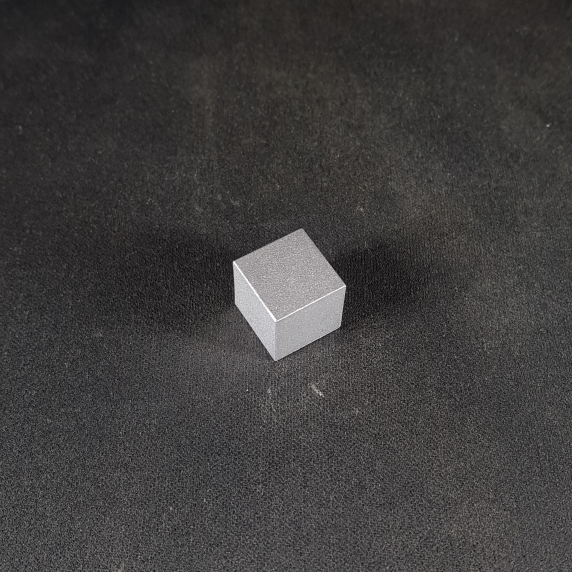
\includegraphics[width=\textwidth]{figures/202105/original-cube.png}
         \caption{Original cube image.}
         \label{fig:original-cube-image}
    \end{subfigure}
    \begin{subfigure}[b]{0.49\textwidth}
         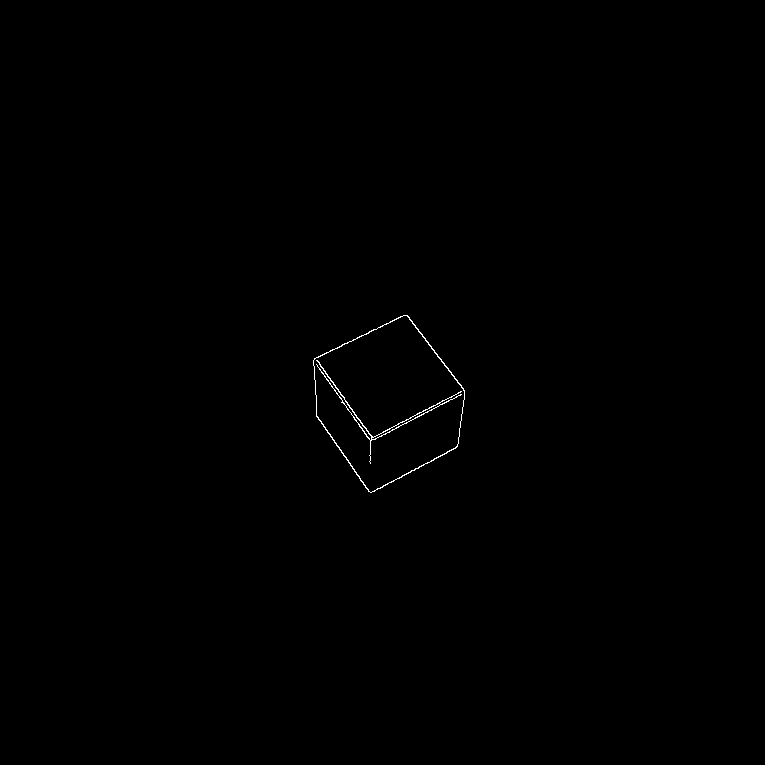
\includegraphics[width=\textwidth]{figures/202105/canny-edge-cube.png}
         \caption{Image output from Canny Edge Detection algorithm.}
         \label{fig:canny-edge-image}
    \end{subfigure}
    \begin{subfigure}[b]{0.49\textwidth}
         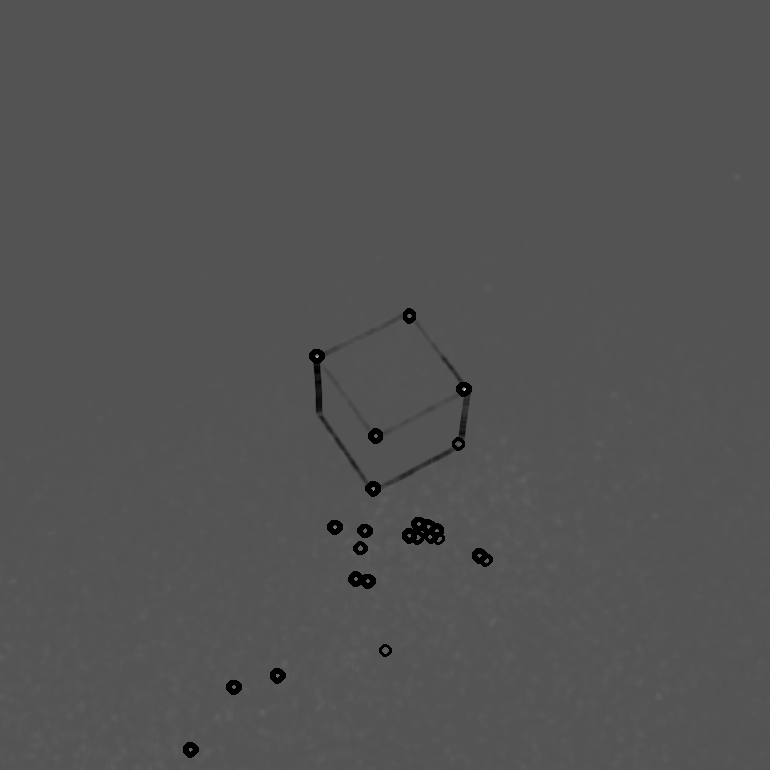
\includegraphics[width=\textwidth]{figures/202105/harris-corner-cube.png}
         \caption{Image output from Harris Corner Detection algorithm.}
         \label{fig:harris-corner-image}
    \end{subfigure}
    \begin{subfigure}[b]{0.49\textwidth}
        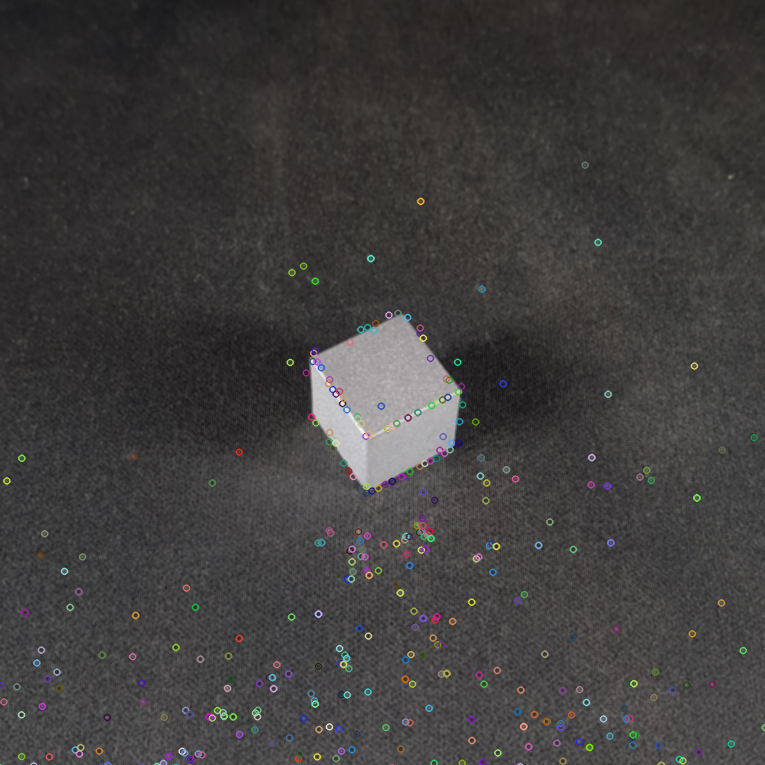
\includegraphics[width=\textwidth]{figures/202105/sift-cube.png}
        \caption{Image output from \ac{SIFT} alogrithm.}
        \label{fig:sift-image}
    \end{subfigure}
    \captionsetup{singlelinecheck = false, justification=justified}
    \caption{Images of a single cube from the same perspective before and after being seperately subjected to edge detection, corner detection and a feature descriptor to isolate features that may be useful in the cube detection process.}
    \label{fig:feature-detectors}
\end{figure}

Detection of an object in a single-view image generally involves the identification of features in the image which can be compared to a template set of features for the desired object to determine its presence and location in the image. Furthermore, certain features may be used in to generate further information about the object beyond feature matching. For example, edges and corners may be used to identify planes which are combined to identify the presence of a cuboid. The first step in this process is to identify what features can be extracted from the image containing a cube that will be useful in detecting the cube. To facilitate this, two LED lights were set up both facing a central point on a plain black surface where a single aluminium construction cube was placed. Multiple photos of the cube with various poses from varying viewpoints were taken with the camera of a Samsung S8 Galaxy smartphone.

The OpenCV C++ library was utilised as the source of various pre-written image processing and machine vision functions required to prototype the feature detection process. Specifically, the Canny Edge Detection, Harris Corner Detection and SIFT feature descriptor implementations were utilised to detect edges, corners and features in the cube images respectively. The OpenCV GUI components were utilised to facilitate the adjustment and tuning of various parameters related to the machine vision functions utilised. This allowed the function to be tuned to produced better results on the cube image dataset. \FigRef{fig:feature-detectors} shows the output of these functions when tuned and applied to the original image of the cube shown in \FigRef{fig:original-cube-image}.

The Canny Edge Detection output shown in \FigRef{fig:canny-edge-image} was the clearest output of the three algorithms. However, the algorithm frequently detected the edges of the fine pattern present on the surface. Image segmentation will be considered to address this issue. The Harris Corner Detection algorithm whose output is shown in \FigRef{fig:harris-corner-image} did not perform as well as the edge detection and needed to have its sensitivity increased significantly to detect most of the cube corners. Lastly, the \ac{SIFT} algorithm output as shown in \FigRef{fig:sift-image} was poor as it identified very few features on the cube itself and the features it did identify were mostly edge features which are less useful. The next computer vision technique I intend to explore in order to supplement the feature descriptor techniques explored so far is image segmentation as the background noise introduced difficulty in tuning the feature descriptors.

\pendsign